\section{Introduction}

Large language model (LLM) agents have become increasingly capable at tool use, code editing, and autonomous problem solving \citep{codeact,alphaevolve,automind}. In software engineering settings, they can inspect repositories, synthesize patches, run tests, and revise their own outputs. Yet the task regime that motivated this work is not the short edit; it is the long task. Long tasks require the agent to keep moving after interruptions, partial failures, context loss, and repeated verification cycles. The dominant interaction pattern remains surprisingly short-lived: a user opens a session, the agent reasons through the current task, local feedback is consumed in the moment, and much of the operational knowledge disappears when the session ends.

Experience-driven agents and procedural memories address parts of this problem by storing trajectories, reflections, workflows, or skills \citep{expel,voyager,awm,memp,legomem,xu2025amemagenticmemoryllm}. These approaches highlight a common insight: capable agents should not rediscover the same behavior every time. Our work arrived at a stronger systems claim: for long tasks, the roadmap becomes as important as the model prompt itself. It is the slow state that preserves what the project is trying to become. Raw transcripts are too noisy for this role, while a single prompt is too brittle to represent both global strategy and local adaptation.

We introduce \systemname{} (\ours), a repository-level pattern for persistent, self-correcting coding agents. \ours{} is implemented as seven loop skills targeting common agent CLIs: Codex, Gemini, Claude, Qwen, Kimi, MiniMax, and Cursor, plus \texttt{moa-loop} for multi-agent orchestration. Each skill follows the same reflective loop: an optimize pass performs a bounded slice of work, a check pass audits the result, the check pass writes local patches, and the next epoch conditions on those patches. The design deliberately mirrors the deep-learning recipe at the orchestration level. The roadmap is the slow backbone, \activestate{} is the fast adapter, check findings are loss signals, and local patches are externalized update directions.

\begin{figure*}[t]
\centering
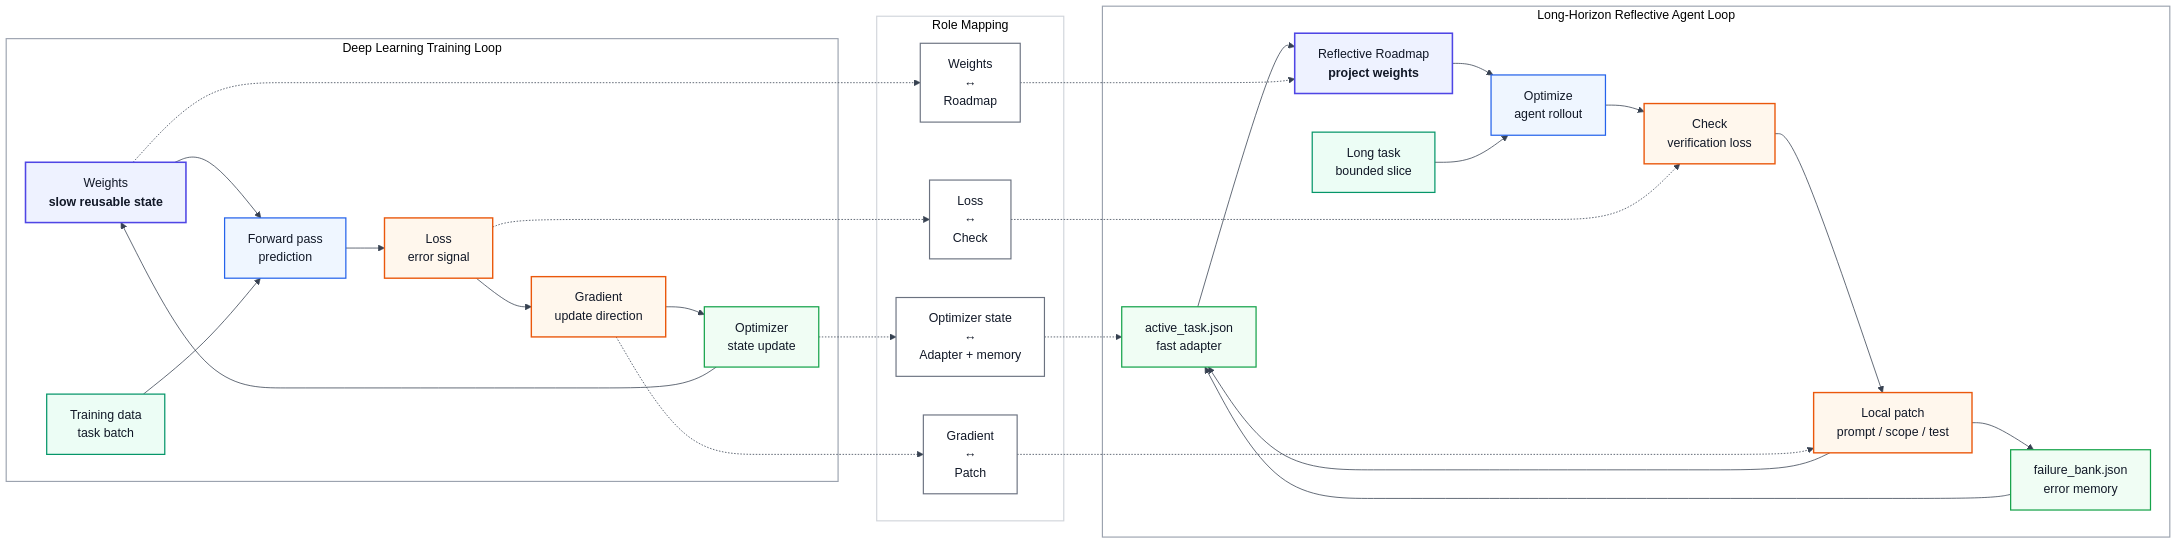
\includegraphics[width=\textwidth]{figures/training-view-agent-loop.png}
\caption{Training view of long-horizon agent loops. \ours{} does not update neural parameters; it imports the training structure into external state. The roadmap is the slow reusable state, while checks, patches, adapters, and failure memory implement a non-parametric update loop.}
\label{fig:overview}
\end{figure*}

Our framing is inspired by machine-learning optimization, but it is explicitly non-parametric. No base model weights are updated. Instead, the system updates external artifacts: roadmaps, task adapters, patches, logs, and failure banks. The analogy is not decorative; it explains why the roadmap matters. Just as pretrained weights carry reusable structure across downstream tasks, the roadmap carries project-level structure across agent epochs. Fast local state can adapt, but it should adapt against the stable backbone rather than rewriting the whole objective.

This paper makes three contributions. First, we formulate long-task coding loops through a roadmap-as-weights abstraction. Second, we describe a concrete seven-CLI implementation that keeps state, logs, and handoffs outside ephemeral chat context. Third, we show how the same abstraction scales to \texttt{moa-loop}: a mixture-of-agents computation graph with vertical serial epochs, horizontal DAG scheduling, and shared blackboard communication.
